% - - - - - - - - - - - - - - - - - - - - - - - - - - - - 
\subsection{PROCM-01 Realizar una venta}

\begin{figure}[htbp]
	\begin{center}
		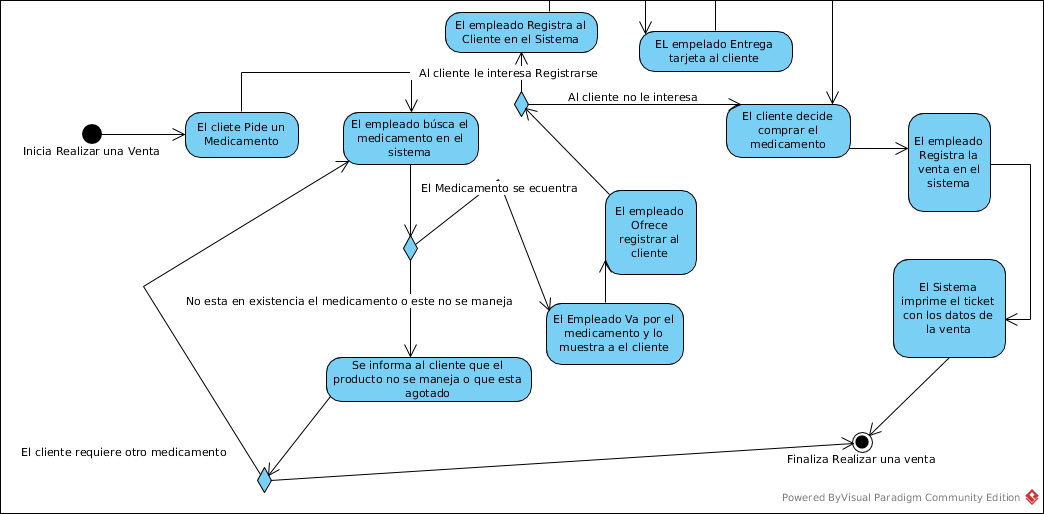
\includegraphics[width=.8\textwidth]{images/TOBERealizarVenta}
		\caption{PROCM-01 Realizar una venta}
		\label{fig:proceso3}
	\end{center}
\end{figure}

\begin{description}
	\item[Descripción:] Ahora con el sistema en función, cuando un cliente venga buscando un medicamento, se le podrá brindar de forma más rápida información de dicho medicamento.
	\item[Entradas:] \cdtEmpty
        \begin{itemize}
			\item nombre del medicamento
			\item ingredientes activos del medicamento.
			\item código de barras del medicamento.
        \end{itemize}
	\item[Salidas:] \cdtEmpty
        \begin{itemize}
			\item Datos del medicamento.
        \end{itemize}	
    \item[Mejoras esperadas:]se ahorra tiempo para la venta, lo cual le conviene al cliente y a la farmacia.
    \item[Casos de uso:] CU 39 Realizar una venta, CU 12 Listar medicamentos, CU33 Listar Clientes, CU 36 Registrar Clientes, CU35 Cambiar datos del cliente, CU 32 Hacer devolución al cliente, CU31 Darle crédito a un cliente, CU30 Aplcar credito de un cliente, CU29 Registrar una venta como devolución, CU25 Reporte de Ventas Por empleado.
\end{description}
